\section{Custom Quantum Gates}

Qiskit let us create our own gates. This can be done by build the desired gate from the basis gate set supplied by the
Qiskit SDK and then invoke the \verb|to_gate()| member method of the circuit object. For example, we can create a new
gate $G$ from the circuit we created from the previous section. After we create the custom gate we can use the \verb|append|
member method to append it to our base circuit.

\begin{figure}[ht]
    \centering
    \begin{minted}{python3}
        from qiskit import QuantumCircuit
            
        example_circuit = QuantumCircuit(2, name="G")
            
        example_circuit.h(0)
        example_circuit.x(1)
            
        example_gate = example_circuit.to_gate()
            
        circuit = QuantumCircuit(2)
            
        circuit.append(example_gate, [0, 1])
        print(circuit.draw("latex_source"))
    \end{minted}
    \centering
    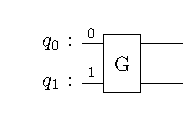
\includegraphics{images/4_Qiskit/example_custom_gate_1.pdf} 
    \caption{Creating a custom gate $G$ and appending it to another circuit}
\end{figure}